\section{Experiments}
\nocite{Kanade2000CK+}\nocite{Lucey2010CK+}

TODO: describe setup of datasets sued for training and validation.Present results

\subsection{Data}
For training a system to recognize facial expression effectively, the dataset should focus on several main expressions including anger, disgust, fear, happiness, sadness and surprise. Moreover, a proper dataset should be composed of faces with kinds of face shapes, colors, facial and scalp hairs from many participants with different genders, ethnic backgrounds and ages. 
\\
\\
The dataset this paper adopted is from the Cohn-Kanade Facial Expression Dataset. The dataset refers to seven emotions including anger, contempt, disgust, fear, happiness, sadness and surprise. There are 5105 images from 123 subjects, who ranged in age from 18 to 30 years. Sixty-five percent are female, eight-five percent are Euro-American and fifteen percent are African-American and Asian. They were observed in an observation room equipped with a chair on which to sit and a camera was located directly in front of the subject. Therefore all images have the uniform background and lighting. The images were digitized into 640*480 or 490 pixel arrays with 8-bit precision for grayscale values and are available in png and jpg. 
\\
\\
In the Cohn-Kanade Facial Expression Dataset, subjects performed a series of several facial displays from neutral expressions to peak expressions and images were taken frame by frame. In order to train a powerful system, we chose neutral faces and obvious expressions. That means there is no indistinguishable expression in our dataset. Figure 1 shows some example of the dataset.



\begin{figure}[h!]
\centering
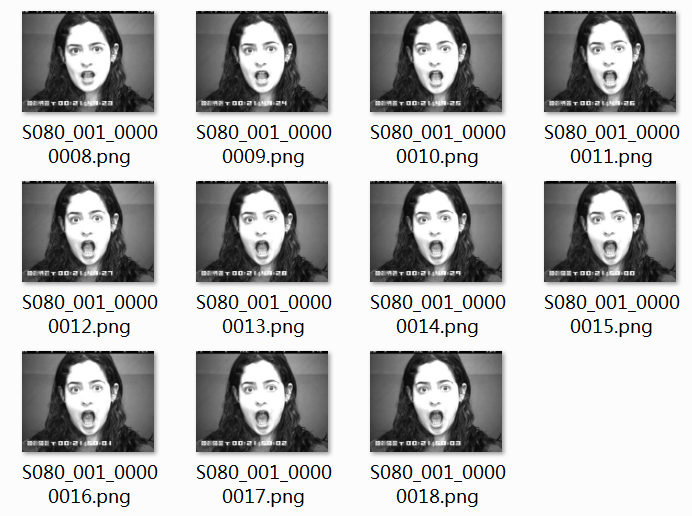
\includegraphics[scale=0.8]{img/example.png}
\caption{Example of dataset}
\label{Example of dataset}
\end{figure}

\subsection{Experiment setup}
The experiments were performed doing one versus all classification. The data for each expression is divided into a training and a validation set and an SVM
classifier is calculated based on the training set. The accuracy of the classifiers is then measured on the validation set. It was ensured that images of the same
person are not present in both the training and validation set. The fraction of the data used for the validation set is a configurable parameter, for the 
following experiments 75\% of the data was used for the training set and 25\% for the valdiation set. 

\subsection{Manually extracted patches}
For this experiment we manually extracted the patches for each eye, the area between the eyes and the mouth region. These regions were chosen because they 
appear to be the most discriminative. The patches were extracted with as uniform alignment as possible and resized to 96 x96 pixels. 
Tables \ref{table:left_eye}, \ref{table:right_eye}, \ref{table:between_eyes} and \ref{table:mouth} show the results for each region, for classifiers trained 
with the original patch size of 96x96 and also rescaled to 32x32 and 64x64 pixels. Shrinking the images on the one hand results in fewer hog features which
is likely to reduce the effect of overfitting, on the other hand some visual information may be lost. The table entries represent the fraction of the
images of the corresponding expression that were correctly classified, in the 0 to 1 range.

%\subsection{Results}

\begin{table}
\caption{Left eye patches}
\label{table:left_eye}

\begin{tabular}{| c | c | c | c |}
\hline
Expression & 32 x 32 &  64 x 64  & 96 x 96  \\

\hline
Angry & 0.5789 & 0.6786 & 0.6767 \\
Contempt & 0.6596 &	0.5745 & 0.5532 \\
Disgust	& 0.7586 &	0.7672 &	0.7651 \\
Fear &	0.6155 & 0.6315 & 0.6394 \\ 
Happy &	0.6063 & 0.6562 & 0.6464 \\ 
Neutral & 0.6851 &	0.6948 & 0.7023 \\
Sadness & 0.5207 & 0.5021 &	0.5 \\
Surprise & 0.7424 &	0.7591 & 0.75 \\

\hline
\end{tabular}
\end{table}

\begin{table}
\caption{Right eye patches}
\label{table:right_eye}

\begin{tabular}{| c | c | c | c |}
\hline
Expression & 32 x 32 &  64 x 64  & 96 x 96  \\

\hline
Angry    & 0.562 & 0.6353 & 0.6617 \\
Contempt & 0.6277 & 0.5106 & 0.617 \\ 
Disgust	 & 0.7263 & 0.7414 & 0.7155 \\
Fear	 & 0.6474 & 0.5992 & 0.5893 \\
Happy	 & 0.6171 & 0.6063 & 0.6573 \\
Neutral  & 0.7065 & 0.7251 & 0.7562 \\
Sadness  & 0.498 & 0.5187 & 0.5436 \\
Surprise & 0.7774 & 0.7866 & 0.7866 \\

\hline
\end{tabular}
\end{table}

\begin{table}
\caption{Part between eyes patches}
\label{table:between_eyes}

\begin{tabular}{| c | c | c | c |}
\hline
Expression & 32 x 32 &  64 x 64  & 96 x 96  \\

\hline
Angry & 0.7971 & 0.812 & 0.7857 \\
Contempt & 0.4468 & 0.4574 & 0.4681 \\
Disgust & 0.6983 & 0.7155 & 0.7306 \\
Fear & 0.7071 & 0.7649 & 0.7351 \\
Happy & 0.8503 & 0.8503 & 0.8329 \\
Neutral & 0.7438 & 0.7845 & 0.7921 \\
Sadness & 0.7324 & 0.7697 & 0.7635 \\
Surprise & 0.7317 & 0.7485 & 0.7165 \\

\hline
\end{tabular}
\end{table}


\begin{table}
\caption{Mouth patches}
\label{table:mouth}

\begin{tabular}{| c | c | c | c |}
\hline
Expression & 32 x 32 &  64 x 64  & 96 x 96  \\

\hline
Angry	&	0.7782	&	0.8008	&	0.7876	\\
Contempt	&	0.6277	&	0.6596	& 0.6596 \\
Disgust	&	0.6897	&	0.7888	&	0.7996	\\
Fear	&	0.7231	&	0.8108	&	0.8068	\\
Happy	&	0.8948	&	0.9111	&	0.9121	\\
Neutral	&	0.7818	&	0.8405	&	0.8204	\\
Sadness	&	0.8589	&	0.8651	&	0.8631	\\
Surprise &	0.8628	&	0.8674	&	0.8959	\\

\hline
\end{tabular}
\end{table}

\subsection{SVM on the entire facial images}
We also experimented with training SVM classifiers considering the entire facial area as a single patch. First the bounding box of the face was detected
for each image using the Viola-Jones algorithm, then rescaled to a uniform size. % TODO: Add Reference. 
The rest of the procedure was identical to the preceding experiment. The results can be found in Table \ref{table:entire_images}.

\begin{table}
\caption{Classifying the whole image}
\label{table:entire_images}

\begin{tabular}{| c | c | c | c |}
\hline
Expression & 32x32 & 96 x 96  \\

\hline
Angry	 & 0.6165 & 0.6015	\\
Contempt & 0.4894 & 0.4043	\\
Disgust	 & 0.7109 & 0.8783	\\
Fear	 & 0.354  & 0.6420	\\
Happy	 & 0.808  & 0.9198	\\
Neutral	 & 0.7203 & 0.8115	\\
Sadness	 & 0.5996 & 0.6432	\\
Surprise & 0.8765 & 0.9436	\\

\hline
\end{tabular}
\end{table}

\section{Discussion}
For the manually extracted patches the best overall results were obtained for the mouth region, with over 80\% of the images classified correctly.
This confirms our intuition as this region is the most distinguishable
from a human perspective. Results for the eye regions were better than expected, as visually the extracted patches look very similar. For the disgust emotion all 
four regions lead to comparable results, while for the anger emotion the region between the eyes is almost as discriminative as the mouth. 
Rescaling the images does not appear to have a very significant effect. 

Performing SVM classification on the entire facial region led to good results if the region was rescaled to 96x96 pixels, better than all manually extracted 
patches except the mouth. In this case there is a clear loss
of precision if the image is rescaled to 32x32 pixels. % TODO Run the experiment without face detection to measure the effect, discuss the original paper



